\documentclass{beamer}

\usepackage{graphicx}
\usepackage{listings}
\usepackage[
	backend=biber,
	style=verbose,
	sorting=ynt
]{biblatex}

\usepackage{derivative}
\usepackage{subfig}
\usepackage{tikz}
\usepackage{pgfplots}
\pgfplotsset{compat=1.18}
\usepackage{amsmath}

\addbibresource{references.bib}

\usetheme{cs}


% Document data for the title page
\title{A Galerkine method for the 1D Helmholtz equation}
\subtitle{An introduction to PDEs and Numerical Mathematics through the example of wave propagation}
\author[V.~de Nodrest]{V.~de Nodrest\inst{1}}
\institute[UFT/VFU]{
  \inst{1} CentraleSupélec, Université Paris Saclay
}
\date{\today}


% Definir o nome do orientador
\newcommand{\advisorname}{\textbf{Orientador:}  Prof. Dr. Nome do Orientador}


% The next block of commands puts the table of contents at the beginning of each section and highlights the current section
\AtBeginSection[]
{
  \begin{frame}
    \frametitle{Table of Contents}
    \tableofcontents[currentsection]
  \end{frame}
}


\begin{document}


\titlegraphic{\logocstext \hspace{2em} \logogretext}

\frame{\titlepage}

% Insert the general toc
\begin{frame}{Table of Contents}
  \tableofcontents    
\end{frame}

\section{First}

\subsection{First first}


\begin{frame}
  \frametitle{The wave equation}

  Many physical problems invole the wave equation, which describes wave propagation in media that are homogeneous, isotropic, linear et non dispersive:

  \begin{block}{The wave equation}
    \vspace{-0.6cm}
    \begin{align*}
      \pdv[2]{p}{t} &= c^2 \Delta p
    \end{align*}
    \vspace{-0.5cm}
  \end{block}

  $\Delta = \nabla^2$ is the Laplacian, a differential operator. \\
  $p$ is a physical phenomenon propagated through one of the aforementioned media at a speed $c$. \\
  It depends on both space $\mathbf{r}$ and time $t$.


\end{frame}


\begin{frame}
  \frametitle{Variable seperation}

  Assuming the solution is separable in time and space ($ p(\mathbf{r}, t) = u(\mathbf{r})T(t) $),
  the wave equation can be rewritten as such:

  \[
    \frac{\Delta u}{u} = \frac{1}{c^2} \odv[2]{T}{t}
  \]

  The left-hand side only depends on space and the right-hand side only depends on time.
  In order to be equal in any situation, both members need to be equal to the same constant.
  This constant is set to $ - k^2 $ for convenience:
  \begin{align*}
    \frac{\Delta u}{u} &= - k^2 \\
    \frac{1}{c^2 T} \odv[2]{T}{t} &= - k^2
  \end{align*}

\end{frame}


\begin{frame}
  \frametitle{The Helmholtz equation}

  Rearranging the first equation (space-dependent) yields:

  \begin{block}{The homogeneous Helmholtz equation}
    \vspace{-0.6cm}
    \begin{align*}
      \Delta u + k^2 u = 0
    \end{align*}
    \vspace{-0.6cm}
  \end{block}

  It is possible to account for sources using $f$,
  a function with compact support, thus yielding:

  \begin{alertblock}{The inhomogeneous Helmholtz equation}
    \vspace{-0.6cm}
    \begin{align*}
      \Delta u + k^2 u = f
    \end{align*}
    \vspace{-0.6cm}
  \end{alertblock}

\end{frame}



\begin{frame}[fragile]
  \frametitle{Our 1D Helmholtz problem}

  We consider the following problem,
  a simple yet telling example of a situation involving the Helmholtz equation:
  \vspace{0.6 cm}
  \begin{alertblock}{Our 1D Helmholtz problem}
    \vspace{-0.6cm}
    \begin{align}
      u'' + k^2 u &= 0 ~ ~ {\text in} ~ ~ ]0, 1[ \\
      u'(0) &= i k \\
      u'(1) &= i k u(1)
    \end{align}
    \vspace{-0.6cm}
  \end{alertblock}

\end{frame}


\begin{frame}[fragile]
  \frametitle{About our problem}

  \begin{block}{Our 1D Helmholtz problem}
    \vspace{-0.6cm}
    \begin{align}
      \setcounter{equation}{0}
      u'' + k^2 u &= 0 ~ ~ {\text in} ~ ~ ]0, 1[ \\
      u'(0) &= i k \\
      u'(1) &= i k u(1)
    \end{align}
    \vspace{-0.6cm}
  \end{block}

  \begin{itemize}
    \item \( u \) is a 1D complex-valued function, at least two times derivable
    \item \(f = 0 \), so this problem "sourceless"/homogeneous in the domain
    \item (2), assigning a value to the derivative, is called a Neumann "flux" boundary condition.
    \item (3), establishing a linear relationship between the value and the derivative, is called a Robin "impedance" boundary condition.
  \end{itemize}

\end{frame}


\begin{frame}[fragile]
  \frametitle{The exact solution}

  The problem can be solved with linear PDE tools, yielding an unique solution:

  \begin{block}{The "Euler wave" exact solution}
    \vspace{-0.6cm}
    \begin{align*}
      \forall x \in [0, 1], ~ u(x) &= e^{ikx}
    \end{align*}
    \vspace{-0.6cm}
  \end{block}

  Our problem is a simple case of a well-posed problem.

  \begin{figure}
    \centering
    \subfloat[3D complex plot\label{fig:1a}]{
      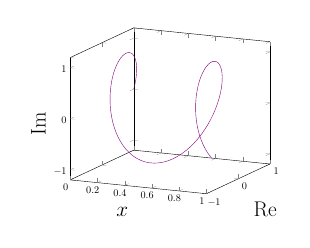
\begin{tikzpicture}[scale=0.37]
        \begin{axis}[
            view={25}{15},
            xlabel={\huge $x$},
            ylabel={\huge Re},
            zlabel={\huge Im},
        ]
          \addplot3+ [
              color=violet,
              domain=0:1,        % Changed: x from 0 to 1
              samples=100,       % Changed: more samples for smoothness
              samples y=1,
              mark=none,         % Added: removes the beads/markers
          ] (
              {x},
              {cos(deg(10*x))},  % Changed: x instead of \x, deg() for radians
              {sin(deg(10*x))}   % Changed: x instead of \x, deg() for radians
          );
      \end{axis}
    \end{tikzpicture}
    }
    \qquad
    \subfloat[Real part\label{fig:1b}]{
      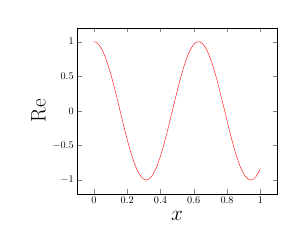
\begin{tikzpicture}[scale=0.37]
        \begin{axis}[
          xlabel={\huge $x$},
          ylabel={\huge Re},
        ]
          \addplot [
            color=red,
            domain=0:1,
            samples=100,
            mark=none,
          ] {
            cos(deg(10*x))
          };
        \end{axis}
      \end{tikzpicture}
    }
    \qquad
    \subfloat[Imaginary part\label{fig:1c}]{
      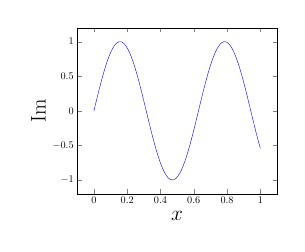
\begin{tikzpicture}[scale=0.37]
        \begin{axis}[
          xlabel={\huge $x$},
          ylabel={\huge Im}
        ]
          \addplot[
            color=blue,
            domain=0:1,
            samples=100,
            mark=none,
          ]{
            sin(deg(10*x))
          };
        \end{axis}
      \end{tikzpicture}
    }
  \label{fig:1}
  \caption{Exact solution with $k = 10$}
  \end{figure}

\end{frame}


\begin{frame}[fragile]
  \frametitle{Weak formulation (1)}

  Let's forget about our exact solution and apply conventional PDE tools,
  which are mandatory for harder problems and for the Galerkine methods. \\
  \vspace{0.6 cm}
  We will assume that $u$ exists and is in $V = H^2(0,1)$
  ($u$ is two times derivable and $u$, $u'$ and $u''$ can all be squared than integrated over $]0,1[$). \\
  \vspace{0.6 cm}
  Then we must have, for every $v$ in $V$:
  $$
  \int_{]0,1[}^{} u'' \overline{v} + k^2 \int_{]0,1[}^{} u \overline{v} = 0
  $$



\end{frame}


\begin{frame}[fragile]
  \frametitle{Weak formulation (2)}

  Integrating by parts and noting $\langle u, v \rangle_{L^2} = \int_{]0,1[}^{} u \overline{v}$, we get:
  \begin{block}{Our weak formulation}
    \vspace{-0.6cm}
    \begin{align*}
      \forall v \in V, ~ k^2 \langle u, v \rangle_{L^2} - \langle u', v' \rangle_{L^2} +  ik \left[ u(1) \overline{v(1)} - \overline{v(0)} \right] &= 0
    \end{align*}
    \vspace{-0.6cm}
  \end{block}

  This is only one of the many possible weak formulations we could have obtained.
  Other choices could have been made regarding:
  \begin{itemize}
    \item The space to which $u$ belongs (test functions)
    \item The space to which $v$ belongs (weighting functions)
    \item The norm and the scalar product
  \end{itemize}


\end{frame}


\begin{frame}[fragile]
  \frametitle{Variational formulation (1)}

  We need to rewrite our weak formulation in the standardized form:
  \begin{alertblock}{Variational formulation}
    Find $u \in V_1$ such that
    \vspace{-0.3cm}
      \begin{align*}
        \forall v \in V_2, ~ a(u, v) = l(v)
      \end{align*}
      \vspace{-0.6cm}
  \end{alertblock}  
  Where:
  \begin{itemize}
    \item $V_1$ and $V_2$ are Hilbert spaces (with their respective scalar products)
    \item $a$ is sesquilinear (bilinear in $\mathbb{R}$)
    \item $l$ is antilinear (linear in $\mathbb{R}$)
  \end{itemize}

\end{frame}


\begin{frame}[fragile]
  \frametitle{Variational formulation (2)}

  First, note that $(V, \langle ., . \rangle_{L^2})$ is a Hilbert space. \\
  Based on the weak formulation, we deduce our forms:
  \begin{block}{Our sesquilinear form}
  \vspace{-0.6cm}
    \begin{align*}
      a : V \times V &\longrightarrow \mathbb{C} \\
      (u, v) &\longmapsto k^2 \langle u, v \rangle_{L^2} - \langle u', v' \rangle_{L^2} +  ik \left[ u(1) \overline{v(1)} \right]
    \end{align*}
    \vspace{-0.6cm}
  \end{block}

  \begin{alertblock}{Our antilinear form}
    \vspace{-0.6cm}
      \begin{align*}
        l : V &\longrightarrow \mathbb{C} \\
        v &\longmapsto ik \left[ \overline{v(0)} \right]
      \end{align*}
      \vspace{-0.6cm}
    \end{alertblock}

\end{frame}


\begin{frame}[fragile]
  \frametitle{Continuity of the sesquilinear form}
\end{frame}


\begin{frame}[fragile]
  \frametitle{Continuity of the antilinear form}
\end{frame}


\begin{frame}[fragile]
  \frametitle{Coercivity of the bilinear form}
\end{frame}


\begin{frame}[fragile]
  \frametitle{Lax-Milgram and Fredholm theory}
\end{frame}


\begin{frame}[fragile]
  \frametitle{Galerkin equation}

  Straightforward numerical solving of the variational formulation is not possible,
  as there are infinitely many possible trial functions and weighting functions.\\
  We discretize those spaces, thus yielding:
  \begin{alertblock}{Galerkin equation}
    Find $u \in V_{1}^{h}$ such that
    \vspace{-0.3cm}
      \begin{align*}
        \forall v \in V_{2}^{h}, ~ a(u, v) = l(v)
      \end{align*}
      \vspace{-0.6cm}
  \end{alertblock}  
  Where $V_{1}^{h} \subset V_1$ and $V_{2}^{h} \subset V_2$ are finite.\\
  Be reminded that in our case, $V_1 = V_2 = H^2(0,1)$.\\
  One might notice that the error is orthogonal to the subspaces: 
  $$
  a(u - u^h, v^h) = a(u, v^h) - a(u^h, v^h) = f(v^h) -f(v^h) = 0
  $$
\end{frame}


\begin{frame}[fragile]
  \frametitle{Matrix form of the Galerkin equation}
\end{frame}


\begin{frame}[fragile]
  \frametitle{Galerkin properties}
\end{frame}


  
\section{Bibliography}
  
\begin{frame}[t,allowframebreaks]
  \frametitle{Bibliography}
  \printbibliography
\end{frame}

\end{document}